\documentclass[a4]{article}
\pagestyle{myheadings}

%%%%%%%%%%%%%%%%%%%
% Packages/Macros %
%%%%%%%%%%%%%%%%%%%
\usepackage{mathrsfs}


\usepackage{fancyhdr}
\pagestyle{fancy}
\lhead{}
\chead{}
\rhead{}
\lfoot{}
\cfoot{} 
\rfoot{\normalsize\thepage}
\renewcommand{\headrulewidth}{0pt}
\renewcommand{\footrulewidth}{0pt}
\newcommand{\RomanNumeralCaps}[1]
{\MakeUppercase{\romannumeral #1}}

\usepackage{amssymb,latexsym}  % Standard packages
\usepackage[utf8]{inputenc}
\usepackage[russian]{babel}
\usepackage{MnSymbol}
\usepackage{amsmath,amsthm}
\usepackage{indentfirst}
\usepackage{graphicx}%,vmargin}
\usepackage{graphicx}
\graphicspath{{pictures/}} 
\usepackage{verbatim}
\usepackage{color}



\DeclareGraphicsExtensions{.pdf,.png,.jpg}% -- настройка картинок

\usepackage{epigraph} %%% to make inspirational quotes.
\usepackage[all]{xy} %for XyPic'a
\usepackage{color} 
\usepackage{amscd} %для коммутативных диграмм


\newtheorem{Lemma}{Лемма}[section]
\newtheorem{Proposition}{Предложение}[section]
\newtheorem{Theorem}{Теорема}[section]
\newtheorem{Corollary}{Следствие}[section]
\newtheorem{Remark}{Замечание}[section]
\newtheorem{Definition}{Определение}[section]
\newtheorem{Designations}{Обозначение}[section]




%%%%%%%%%%%%%%%%%%%%%%%% 
%Сношение с оглавлением% 
%%%%%%%%%%%%%%%%%%%%%%%% 
\usepackage{tocloft} 
\renewcommand{\cftdotsep}{2} %частота точек
\renewcommand\cftsecleader{\cftdotfill{\cftdotsep}}
\renewcommand{\cfttoctitlefont}{\hspace{0.38\textwidth} \LARGE\bfseries} 
\renewcommand{\cftsecaftersnum}{.}
\renewcommand{\cftsubsecaftersnum}{.}
\renewcommand{\cftbeforetoctitleskip}{-1em} 
\renewcommand{\cftaftertoctitle}{\mbox{}\hfill \\ \mbox{}\hfill{\footnotesize Стр.}\vspace{-0.5em}} 
\renewcommand{\cftsubsecfont}{\hspace{1pt}} 
\renewcommand{\cftparskip}{3mm} %определяет величину отступа в оглавлении
\setcounter{tocdepth}{5} 




\addtolength{\textwidth}{0.7in}
\textheight=630pt
\addtolength{\evensidemargin}{-0.4in}
\addtolength{\oddsidemargin}{-0.4in}
\addtolength{\topmargin}{-0.4in}

\newcommand{\empline}{\mbox{}\newline} 
\newcommand{\likechapterheading}[1]{ 
	\begin{center} 
		\textbf{\MakeUppercase{#1}} 
	\end{center} 
	\empline} 

\makeatletter 
\renewcommand{\@dotsep}{2} 
\newcommand{\l@likechapter}[2]{{\bfseries\@dottedtocline{0}{0pt}{0pt}{#1}{#2}}} 
\makeatother 
\newcommand{\likechapter}[1]{ 
	\likechapterheading{#1} 
	\addcontentsline{toc}{likechapter}{\MakeUppercase{#1}}} 





\usepackage{xcolor}
\usepackage{hyperref}
\definecolor{linkcolor}{HTML}{000000} % цвет ссылок
\definecolor{urlcolor}{HTML}{AA1622} % цвет гиперссылок

\hypersetup{pdfstartview=FitH,  linkcolor=linkcolor,urlcolor=urlcolor, colorlinks=true}



\def \newstr {\medskip \par \noindent} 



\begin{document}
	\def\contentsname{\LARGE{Содержание}}
	\thispagestyle{empty}
	\begin{center} 
		\vspace{2cm} 
		{\Large \sc Санкт-Петербургский Политехнический Университет}\\
		\vspace{2mm}
		{\Large\sc им. Петра Великого}\\
		\vspace{1cm}
		{\large \sc Институт прикладной математики и механики\\ 
			\vspace{0.5mm}
			\textsc{}}\\ 
		\vspace{0.5mm}
		{\large\sc Кафедра $"$Прикладная математика$"$}\\
		\vspace{15mm}
		
		
		{\sc \textbf{Отчёт по\\
			Курсовой работе\\
			по дисциплине\\
			"Математическая статистика"}
			\vspace{6mm}
			
		}
		\vspace*{2mm}
		
		
		\begin{flushleft}
			\vspace{4cm}
			\sc Выполнил студент:\\
			\sc Мальцов Дмитрий Дмитриевич\\
			\sc группа: 3630102/70401\\
			\vspace{1cm}
			\sc Проверил:\\
			\sc к.ф-м.н., доцент\\
			\sc Баженов Александр Николаевич
			\vspace{20mm}
		\end{flushleft}
	\end{center} 
	\begin{center}
		\vfill {\large\textsc{Санкт-Петербург}}\\ 
		2020 год
	\end{center}
	
	\newpage
	\pagestyle{plain}
	

	\newpage
	\tableofcontents{}
	\newpage
	\listoffigures
	\newpage
	
	
	\section{Постановка задачи}
	Имеется датасет проб, содержащий информацию о концентрации определенных химических соединений в каждой из проб.\\
	
	Цель работы: Отпределить, возможно ли разделить данные пробы на две группы.\\
	
	Задачи: Построить метод главных компонент, кластеризировать исходные данные.
	
	
	\section{Подготовка данных}
	Данные представлены в виде двух .xlsx файлов.\\
	Объеденим эти файлы в один, предварительно удалив из них лишнюю информацию. \\
	\begin{figure}[h!]
		\includegraphics[width=\textwidth]{input_data.png}\caption[Пример исходных и очищенных данных]{Пример исходных и очищенных данных}
	\end{figure}
	
	После этого можно считать данные с помощью пакета pandas в Python.
	
	\section{Метод главных компонент}
	\subsection{Описание метода}
		Principal component analysis, PCA - один из основных способов уменьшить размерность данных, потеряв наименьшее количество информации. PCA применяется к данным, записанным в виде матрицы. Суть метода заключается в том, что из исходной матрицы мы получаем матрицу главных компонент меньшего размера, где каждый столбец(главная компонента) объясняет дисперсию исходных данных. Чем больше главных компонент мы берем, тем меньше данных мы теряем, и наоборот.\\
		
		Перед использованием метода данные необходимо отцентрировать и отнормировать. В результате применения этого метода мы приходим от большого количества переменных к новому представлению, размерность которого значительно меньше.  \\
		
		Метод сводится к вычислению сингулярного разложения исходной матрицы либо к вычислению собственных векторов и собственных значений ковариационной матрицы исходных данных. \\
		
		В данной работе было реализовано сингулярное разложение матрицы, затем правильность разложения проверилось с помощью метода PCA, реализованным в программном пакете sklearn.decomposition в python
		%%%$X$ размерности $n\times m$ на две матрицы: \\
		%%%$X = \sum_{i=1}^n t_i p_i^t + E = TP^t + E$, где $t_i = p_{i1} x_1 + ... + p_{im} x_m$
	
	\subsection{Использование сторонних пакетов}
	Применим PCA, для двух главных компонент. Построим график долей объясненной дисперсии для каждой компоненты.
	\begin{figure}[h!]
		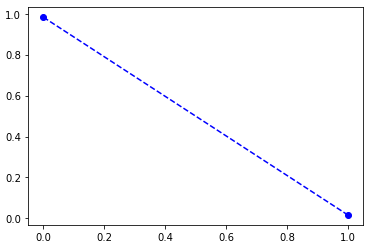
\includegraphics[width=\textwidth]{disp.png}\caption[Доля объясненной дисперсии для каждой компоненты]{Доля объясненной дисперсии для каждой компоненты}
	\end{figure}\\
	Из графика видно, что первая компонента практически полностью объясняет дисперсию исходных данных, поэтому брать больше двух компонент не имеет никакого смысла. Ниже, при риализации МГК через сингулярное разложение мы тоже будем брать первые две главные компоненты.
	\subsection{Сингулярное разложение матрицы}
	Пусть матрица $M$ порядка $m\times n$ состоит из элементов из поля $K$, где $K$ — поле вещественных чисел. \\
	Неотрицательное вещественное число $\sigma$  называется сингулярным числом матрицы $M$ тогда и только тогда, когда существуют два вектора единичной длины $u\in K^{m}$ и $v\in K^{n}$ такие, что:
	$ Mv=\sigma u$ и $M^{*}u=\sigma v$.
	Такие векторы $u$ и $v$ называются левым сингулярным вектором и правым сингулярным вектором, соответствующим сингулярному числу $\sigma$ .\\
	Сингулярным разложением матрицы $M$ порядка $m\times n$ является разложение следующего вида:
	$M=U\Sigma V^{*},$
	где $\Sigma$  — матрица размера $m\times n$ с неотрицательными элементами, у которой элементы, лежащие на главной диагонали — это сингулярные числа (а все элементы, не лежащие на главной диагонали, являются нулевыми), а матрицы $U$ (порядка $m$) и $V$ (порядка $n$) — это две унитарные матрицы, состоящие из левых и правых сингулярных векторов соответственно (а $V^*$ — это сопряжённо-транспонированная матрица к $V$).
	\subsection{Реализация сингулярного разложения}
	Для начала нормализуем исходные данные, при применении PCA из sklearn.decomposition мы этого не делали, так как в данном методе нормализация уже реализована.\\
	
	Затем проведем полное сингулярное разложение. Полное в том смысле, что матрица $vt$ содержит все столбцы исходной матрицы.\\
	
	Далее проверим правильность разложения: для этого поэлементно вычтим из матрицы $X_{svd} = U\Sigma V^{*}$ элементы исходной матрицы, возведем в квадрат и подсчитаем сумму полученных элементов. В итоге мы получили число близкое к нулю, значит разложение было произведено верно.
	
	\subsection{Проверка сингулярного разложения}
	Теперь проверим полученную матрицу главных компонент: для этого умножим исходную нормализованную матрицу данных на транспононированную матрицу двух первых столбцов матрицы главных компонент $V^*$ и сраним со значениями, полученных при применении  PCA из sklearn.decomposition.
	\begin{figure}[h!]
		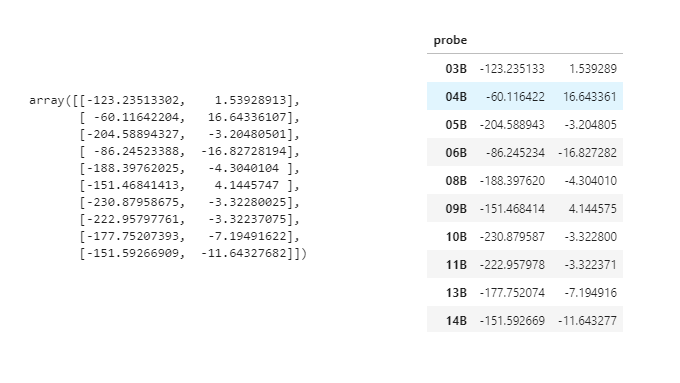
\includegraphics[width=\textwidth]{2PC.png}\caption[Первые 10 элементов матриц гланых компонент. Слева-полученные с помощью sklearn, справа-полученные через сингулярное разложение]{Первые 10 элементов матриц гланых компонент. Слева-полученные с помощью sklearn, справа-полученные через сингулярное разложение}
	\end{figure} \\

	Также построим полученные матрицы и сравним визуально. Видим, что матрицы и графики совпали, значит разложение произведено верно и МГК действительно сводится к сингулярному разложению.
	\begin{figure}[h!]
		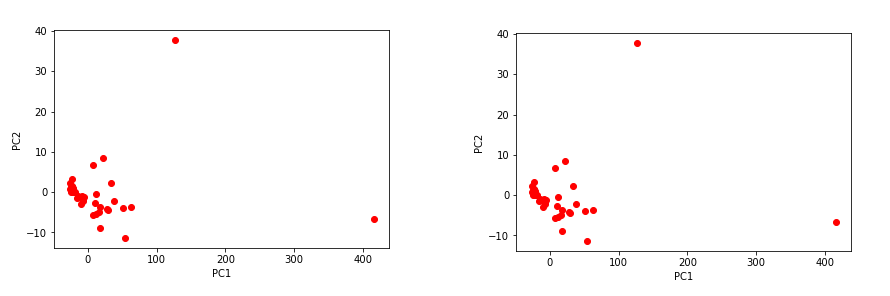
\includegraphics[width=\textwidth]{out.png}\caption[Распределение данных полученных с помощью встроенного PCA и с помощью сингулярного разложения]{Распределение данных полученных с помощью встроенного PCA и с помощью сингулярного разложения}
	\end{figure} \\

	
	\section{Кластеризация полученных данных}
	\subsection{Использованные методы}
	Для кластеризации данных используем два метода: классический KMeans и DBSCAN из sklearn.cluster
	\subsection{Результаты кластеризации}
	KMeans сумел кластеризировать данные на две группы, в то время как DBSCAN не смог разделить данные.
	произведено верно и МГК действительно сводится к сингулярному разложению.
	\begin{figure}[h!]
		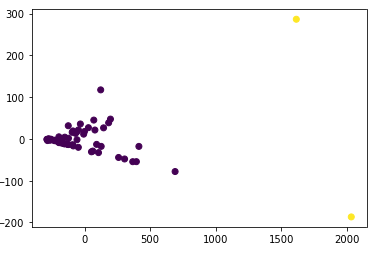
\includegraphics[width=\textwidth]{kmeans.png}\caption[Результат кластеризации с помощью KMeans]{Результат кластеризации с помощью KMeans}
	\end{figure}
	\begin{figure}[h!]
		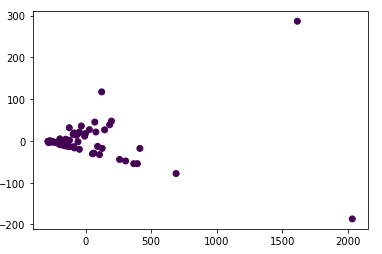
\includegraphics[width=\textwidth]{dbscan.png}\caption[Результат кластеризации с помощью DBSCAN]{Результат кластеризации с помощью DBSCAN}
	\end{figure} \\
	Значения второй группы, полученной с помощью KMeans можно скорее отнести к выбросам, чем к отдельному кластеру. Таким образом, делаем вывод, что исходные данные не получилось разделить по двум группам.
	
	Действительно, для более наглядной демонстрации невозможности разделения данных на две группы построим все графики зависимостей параметров исходных данных друг от друга.\\
	\begin{figure}[h!]
		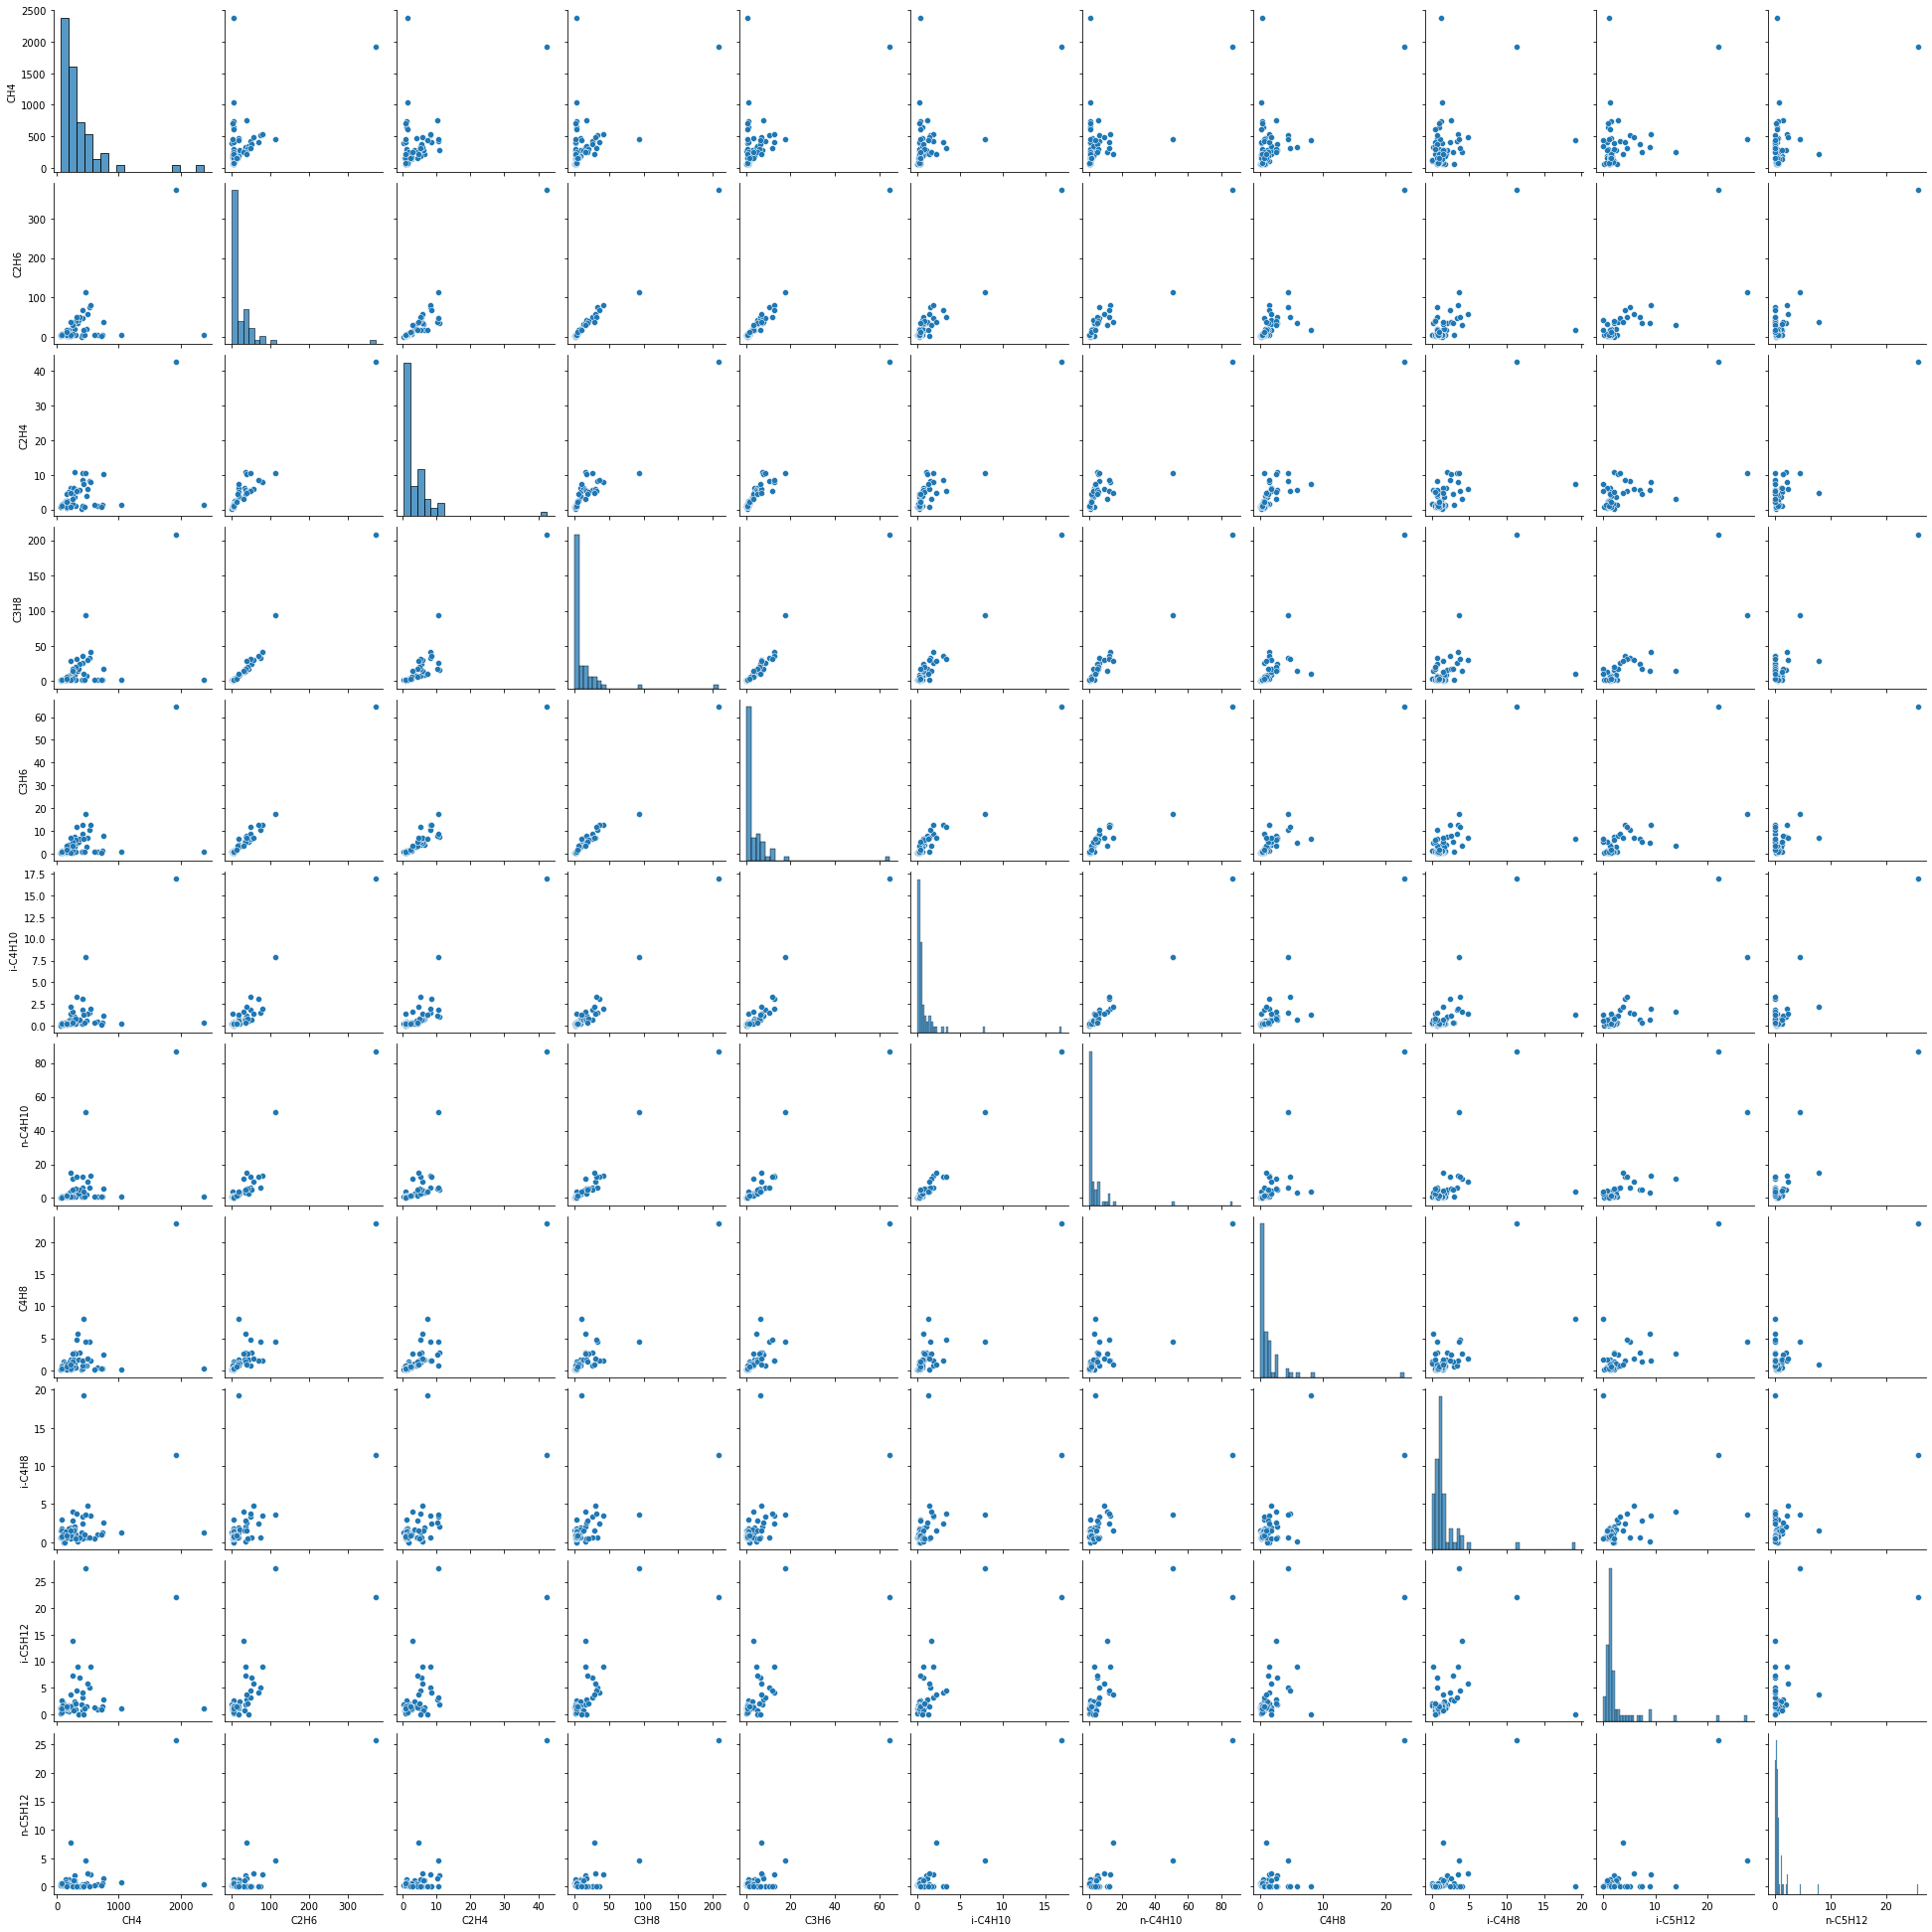
\includegraphics[width=\textwidth]{data_disp.png}\caption[Распределение исходных данных]{Распределение исходных данных}
	\end{figure} 
	Видим, что нигде нет и намека на разделение на группы:\\
	
	\newpage
	\section{Вывод}
	
	При помощи PCA удалось уменьшить размерность до двумерной, так как было обнаружено, что основной вклад в дисперсию исходных данных оказывают первые две компоненты. \\
	
	Было продеманстрировано, что МГК сводится к сингулярному разложению. \\
	
	Тем ни менее, исходные данных оказались слишком похожи, и их не удалось кластеризировать на две группы ни одним из использованных алгоритмов кластеризации.

		\newpage
	\section{Список литературы}
	[1]\href{https://ru.wikipedia.org/wiki/%D0%9C%D0%B5%D1%82%D0%BE%D0%B4_%D0%B3%D0%BB%D0%B0%D0%B2%D0%BD%D1%8B%D1%85_%D0%BA%D0%BE%D0%BC%D0%BF%D0%BE%D0%BD%D0%B5%D0%BD%D1%82#:~:text=%D0%9C%D0%B5%D1%82%D0%BE%D0%B4%20%D0%B3%D0%BB%D0%B0%D0%B2%D0%BD%D1%8B%D1%85%20%D0%BA%D0%BE%D0%BC%D0%BF%D0%BE%D0%BD%D0%B5%D0%BD%D1%82%20(%D0%B0%D0%BD%D0%B3%D0%BB.,%D0%B4%D0%B0%D0%BD%D0%BD%D1%8B%D1%85%2C%20%D0%BF%D0%BE%D1%82%D0%B5%D1%80%D1%8F%D0%B2%20%D0%BD%D0%B0%D0%B8%D0%BC%D0%B5%D0%BD%D1%8C%D1%88%D0%B5%D0%B5%20%D0%BA%D0%BE%D0%BB%D0%B8%D1%87%D0%B5%D1%81%D1%82%D0%B2%D0%BE%20%D0%B8%D0%BD%D1%84%D0%BE%D1%80%D0%BC%D0%B0%D1%86%D0%B8%D0%B8.&text=%D0%9F%D1%80%D0%B8%D0%BC%D0%B5%D0%BD%D1%8F%D0%B5%D1%82%D1%81%D1%8F%20%D0%B2%D0%BE%20%D0%BC%D0%BD%D0%BE%D0%B3%D0%B8%D1%85%20%D0%BE%D0%B1%D0%BB%D0%B0%D1%81%D1%82%D1%8F%D1%85%2C%20%D0%B2,%D1%81%D0%B6%D0%B0%D1%82%D0%B8%D1%8F%20%D0%B4%D0%B0%D0%BD%D0%BD%D1%8B%D1%85%2C%20%D0%B2%20%D0%BE%D0%B1%D1%89%D0%B5%D1%81%D1%82%D0%B2%D0%B5%D0%BD%D0%BD%D1%8B%D1%85%20%D0%BD%D0%B0%D1%83%D0%BA%D0%B0%D1%85.}{Метод главных компонент} \\
	
	[2]\href{https://numpy.org/}{Модуль numpy} \\
	
	[3]\href{https://matplotlib.org/}{Модуль matplotlib} \\

	[4]\href{https://scikit-learn.org/stable/modules/generated/sklearn.decomposition.PCA.html}{Документация sklearn PCA} \\
	
	[5]\href{https://medium.com/@rrfd/standardize-or-normalize-examples-in-python-e3f174b65dfc}{Нормализация и стандартизация в Python} \\
	
	[6]\href{https://habr.com/ru/post/304214/}{Принцип работы МГК} \\
	
	\section{Приложение}
	
	\href{https://github.com/dmitry-maltsov/PolyMatStat/blob/master/Course%20project/research/PCA.ipynb}{Код работы} \\
	
\end{document}